\documentclass[tikz,border=2pt]{standalone}
\usepackage{fontspec}
\IfFontExistsTF{Times New Roman}{\setmainfont{Times New Roman}}{\setmainfont{Tinos}}
\usepackage{unicode-math}
\setmathfont{STIXTwoMath-Regular.otf}
\usetikzlibrary{arrows.meta}

\definecolor{ink}{HTML}{253139}
\definecolor{blueink}{HTML}{52758A}
\definecolor{guidegray}{HTML}{AEBBC4}
\definecolor{framegray}{HTML}{C9D2D8}
\tikzset{
  font=\fontsize{10}{12}\selectfont,
  text=ink,
  track/.style={line width=.85pt,draw=ink},
  guide/.style={line width=.45pt,densely dashed,draw=guidegray},
  op/.style={circle,draw=ink,fill=white,inner sep=0pt,
    minimum size=4.6pt,line width=.7pt},
  cl/.style={circle,draw=ink,fill=ink,inner sep=0pt,
    minimum size=4.6pt,line width=.7pt},
  small/.style={font=\fontsize{9}{11}\selectfont},
  head/.style={font=\fontsize{10.5}{12}\selectfont\bfseries,text=blueink},
  tail/.style={-{Stealth[length=4.4pt,width=4.6pt]}}
}

\begin{document}
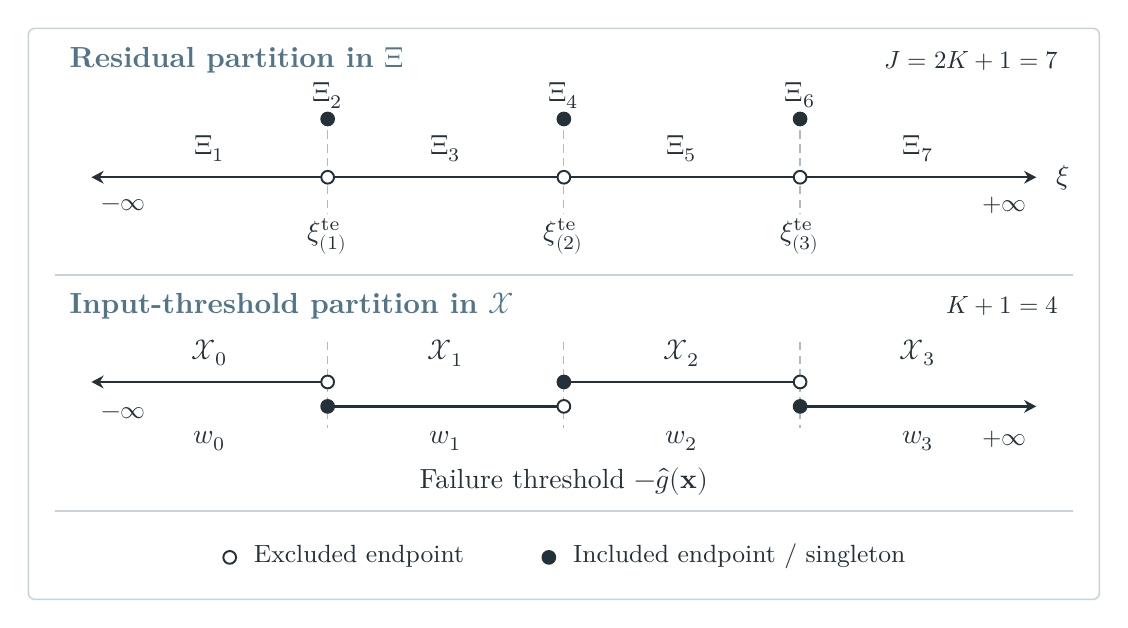
\begin{tikzpicture}[x=1cm,y=1cm]
% Schematic spacing, not observed residual values. All cell definitions match
% manuscript.tex: residual singleton/open cells and left-closed input cells.
\draw[draw=framegray,line width=.55pt,rounded corners=2.2pt]
  (0,0) rectangle (13.6,7.25);
\draw[draw=framegray,line width=.45pt] (.34,4.12)--(13.26,4.12);
\draw[draw=framegray,line width=.45pt] (.34,1.12)--(13.26,1.12);

% Residual partition: the separate singleton markers preserve the atoms.
\node[head,anchor=west] at (.40,6.84) {Residual partition in $\Xi$};
\node[small,anchor=east] at (13.20,6.84) {$J=2K+1=7$};
\foreach \x in {3.80,6.80,9.80}
  \draw[guide] (\x,6.13)--(\x,4.44);
\draw[track,tail] (3.80,5.36)--(.80,5.36);
\draw[track] (3.80,5.36)--(6.80,5.36);
\draw[track] (6.80,5.36)--(9.80,5.36);
\draw[track,tail] (9.80,5.36)--(12.80,5.36);
\foreach \x/\j in {2.30/1,5.30/3,8.30/5,11.30/7}
  \node at (\x,5.72) {$\Xi_{\j}$};
\foreach \x/\j/\k in {3.80/2/1,6.80/4/2,9.80/6/3} {
  \node[op] at (\x,5.36) {};
  \node[cl] at (\x,6.10) {};
  \node at (\x,6.40) {$\Xi_{\j}$};
  \node[fill=white,inner sep=1.7pt] at (\x,4.61) {$\xi_{(\k)}^{\mathrm{te}}$};
}
\node[small,anchor=west] at (.80,5.01) {$-\infty$};
\node[small,anchor=east] at (12.80,5.01) {$+\infty$};
\node[anchor=west] at (12.93,5.36) {$\xi$};

% Input partition: each finite interval includes its left endpoint and
% excludes its right endpoint. Alternating tracks keep both markers visible.
\node[head,anchor=west] at (.40,3.72) {Input-threshold partition in $\mathcal X$};
\node[small,anchor=east] at (13.20,3.72) {$K+1=4$};
\foreach \x in {3.80,6.80,9.80}
  \draw[guide] (\x,3.27)--(\x,2.18);
\draw[track,tail] (3.80,2.76)--(.80,2.76);
\draw[track] (3.80,2.45)--(6.80,2.45);
\draw[track] (6.80,2.76)--(9.80,2.76);
\draw[track,tail] (9.80,2.45)--(12.80,2.45);
\node[op] at (3.80,2.76) {};
\node[cl] at (3.80,2.45) {};
\node[op] at (6.80,2.45) {};
\node[cl] at (6.80,2.76) {};
\node[op] at (9.80,2.76) {};
\node[cl] at (9.80,2.45) {};
\foreach \x/\i in {2.30/0,5.30/1,8.30/2,11.30/3} {
  \node at (\x,3.13) {$\mathcal X_{\i}$};
  \node at (\x,2.01) {$w_{\i}$};
}
\node[small,anchor=west] at (.80,2.36) {$-\infty$};
\node[small,anchor=east] at (12.80,2.03) {$+\infty$};
\node at (6.80,1.50) {Failure threshold $-\hat g(\symbf{x})$};

% Center the complete legend group, including markers and text.
\node[small,anchor=center,inner sep=0pt] at (6.80,.55) {%
  \tikz[baseline=-.45ex]{\node[op] at (0,0) {};}
  \hspace{3pt}Excluded endpoint\hspace{28pt}%
  \tikz[baseline=-.45ex]{\node[cl] at (0,0) {};}
  \hspace{3pt}Included endpoint / singleton};
\end{tikzpicture}
\end{document}
